\documentclass[12pt]{beamer}
\usepackage{listings}
\usepackage{color}
\usepackage{xcolor}
%\usepackage{latexsym}
\usepackage{amsmath}
\usepackage[labelfont=bf]{caption}
\usepackage{graphicx}  %package graphic
\usepackage{siunitx}
\usepackage{tikz}
%\usepackage{algorithmicx}
%\usepackage[noend]{algpseudocode}
\usetikzlibrary{automata, positioning, arrows}
\usetheme{Boadilla}   
\usepackage{xeCJK}
%\usepackage{array}
%\usepackage{tabularx}
%\usepackage{mathtools}
\usepackage{listings}
%\usepackage{textcomp}
\usepackage[T1]{fontenc}
\usepackage{lmodern}
\usepackage{adjustbox}
\usepackage{dirtree}
\usepackage{hyperref}
\usepackage{inconsolata}
\usepackage{textcomp}

\setCJKmainfont{微軟正黑體} 
\sisetup{
	group-separator={,},
	table-number-alignment=right
}


\setbeamerfont{title}{size=\Large,series=\bfseries}  % title size

\setbeamerfont{frametitle}{size=\large,series=\bfseries}  % frametitle size, also can size*=<pt>

\definecolor{themeColor}{rgb}{0.06, 0.3, 0.57}
\usecolortheme[named=themeColor]{structure}

\defbeamertemplate*{footline}{Dan P theme}
{
  \leavevmode%
  \hbox{%
  %\begin{beamercolorbox}[wd=.2\paperwidth,ht=2.25ex,dp=1ex,center]{author in head/foot}%
	%\usebeamerfont{author in head/foot}\insertshortauthor\expandafter\beamer@ifempty\expandafter{\beamer@shortinstitute}{}{~~(\insertshortinstitute)}
  %\end{beamercolorbox}%
  \begin{beamercolorbox}[wd=.7\paperwidth,ht=2.25ex,dp=1ex,center]{title in head/foot}%
	\usebeamerfont{title in head/foot}\insertshorttitle
  \end{beamercolorbox}%
  \begin{beamercolorbox}[wd=.3\paperwidth,ht=2.25ex,dp=1ex,right]{date in head/foot}%
	\usebeamerfont{date in head/foot}\insertshortdate{}\hspace*{2em}
\insertframenumber{} / \inserttotalframenumber\hspace*{2ex} 
  \end{beamercolorbox}}%
  \vskip0pt%
}
\makeatother

% Item include picture
\setbeamertemplate{itemize item}   % First Level item
{
\includegraphics[height=0.33cm]{../Figures/golden-earth-on-white}}

\setbeamertemplate{itemize subitem} % Second level item
{
\includegraphics[height=0.31cm]{../Figures/golden-sun-on-white}}

\setbeamertemplate{itemize subsubitem} % Third Level item
{
\includegraphics[height=0.27cm]{../Figures/golden-paw-on-white}}

\definecolor{darkgold}{rgb}{0.765 0.64 0.0} % for highlighted text in black-and-white slides
\newcommand{\code}[1]{\texttt{#1}}

%\newtheorem{problem}{Problem}
\mode<presentation>{\newtheorem{algorithm}{Algorithm}}
\mode<article>{\newenvironment{algorithm}{}{}}
%\newtheorem{solution}{Solution}

\newlength{\subtextwidth}
\setlength{\subtextwidth}{11cm}

\newenvironment{cbox}{
	\begin{center}
	\begin{tabular}{|l|}
	\hline
	\begin{minipage}[t]{\subtextwidth}}
	{\vspace{.25ex}
	\end{minipage}
	\hline
	\end{tabular}
	\end{center} }

\lstdefinestyle{mystyle}{
	basicstyle=\setmonofont{Consolas},
	columns=fullflexible,
	keepspaces=true,
	upquote=true,
	showstringspaces=false,
	commentstyle=\color{gray},
	keywordstyle=\color{teal},
	identifierstyle=\color{black},
	stringstyle=\color{brown},
	language=C++
}

\lstset{style=mystyle,frame=single,}
\makeatletter
\lst@CCPutMacro
	\lst@ProcessOther {"2A}{%
	%   \lst@ttfamily 
		 {\raisebox{1.5pt}{*}}% used with ttfamily
		%   \textasteriskcentered
		  }% used with other fonts
	\@empty\z@\@empty
\makeatother


\newcommand{\mathdef}[1]{\relax\ifmmode #1\else $#1$\fi}
\newcommand{\true}{\mathdef{\mathit{true}}}
\newcommand{\false}{\mathdef{\mathit{false}}}
\renewcommand{\implies}{\mathdef{\rightarrow}}
\newcommand{\ifonlyif}{\mathdef{\leftrightarrow}}
\newcommand{\entails}{\mathdef{\vdash}}
\newcommand{\PROPS}{\mathdef{\mathit{PROPS}}}
\newcommand{\BOOL}{\mathdef{\mathit{BOOL}}}
\newcommand{\Note}[1]{\textsl{\small(#1)}}

\newcommand{\ultimate}{\textsc{Ultimate }}
\newcommand{\ultimates}{\textsc{Ultimate}'s }
\newcommand{\automizer}{\textsc{Automizer }}
\newcommand{\ultimateURL}{\url{https://monteverdi.informatik.uni-freiburg.de/ultimate}}

\mode<presentation>{\title{Introduction to Utimate}}
\mode<article>{\title{Algorithms 2019: Analysis of Algorithms}}
\subtitle{(Based on [Daniel Dietsch : Automated verification of system requirements and software specifications. 2016.])}
\author{林宏陽}
%\institute[IM.NTU]{Department of Information Management\\ National Taiwan University}
%\date[Algorithms 2019]{\null}
\mode<presentation>{\date[SVVRL]{\null}}
\mode<article>{\date{\today}}

\begin{document}
\begin{frame}
	\maketitle
\end{frame}

\begin{frame}{Ultimate}
  	\begin{itemize}
		\item \ultimate is a modular, plugin-based program analysis framework. It provides a platform for the development of automated program analysis methods that facilitates the reuse of existing components (plugins) and analysis results.
		\item Website : \ultimateURL
		\item Github page : \url{https://github.com/ultimate-pa/ultimate}
	  	\item Installation : Just follow the wiki page on github. \Note{Z3.exe should be updated in Windows.}
	\end{itemize}
\end{frame}

\begin{frame}{Core Architecture and Plugin Lifecycles}
  	\begin{itemize}
		\item The \ultimate framework is based on the Eclipse Rich Client Platform
	(Eclipse RCP).
		\item Eclipse RCP is a software development framework that provides  the ability to load and unload plugins dynamically at runtime and isolate them from each other.
		\item Eclipse RCP is written in the programming language Java.
		Hence, most of \ultimate is also written in Java (currently, Java 11).
  	\end{itemize}
\end{frame}

\begin{frame}{Core Architecture and Plugin Lifecycles (cont'd)}
	\begin{itemize}
	  	\item  In this context, the plugin \code{UltimateCore} provides the interface between Eclipse RCP and all active plugins.
	  	\item  Plugins can be executed one after another in a \textbf{toolchain}. A toolchain is defined by an XML file.
	  	\item \code{UltimateCore} manages different representations of a program analysis problem as \textbf{models} and passes them between active plugins according to the toolchain. The plugins may analyse, transform, or visualize the models they receive.
	\end{itemize}
\end{frame}

\captionsetup[figure]{font=scriptsize ,labelfont=scriptsize}
\begin{frame}{Ultimate toolchain illustration}
    \begin{figure}
        \centering
        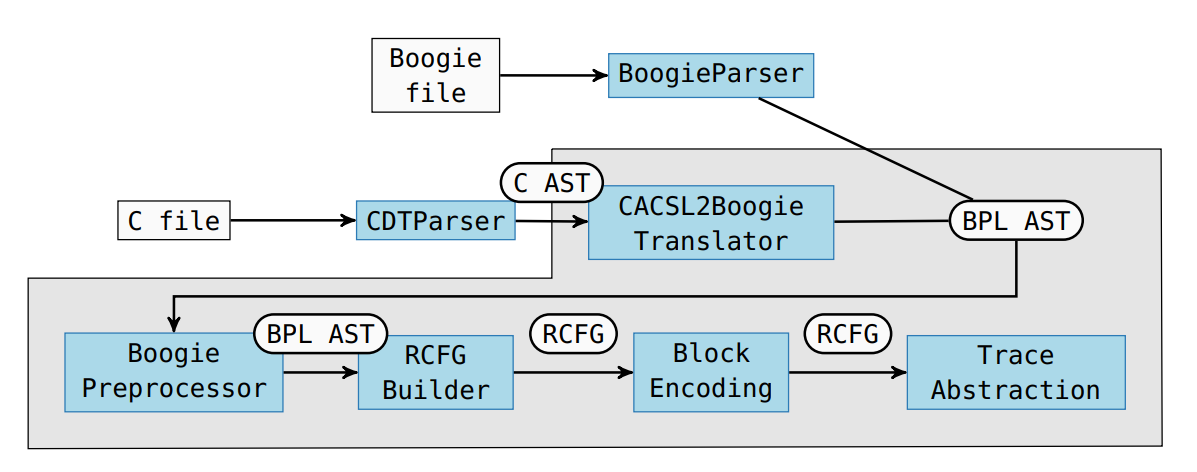
\includegraphics[scale=0.35]{toolchain.png}
        \caption{\ultimate toolchain for the tool \ultimate \automizer. The light boxes are input files, the dark boxes are plugins, the rounded boxes are the internal models that are passed between the plugins, and the shaded area is the toolchain for C programs. Removing the plugin \code{CACSL2BoogieTranslator} from the toolchain defines a new toolchain that can be used to process Boogie programs.
		}
    \end{figure}    
\end{frame}

\begin{frame}{Five Plugin types}
	\begin{itemize}
		\item Plugin types can be used in toolchains
		\begin{itemize}
			\item \textbf{Source} : Source plugins define a file-to-model transformation.
			\item \textbf{Analyzer and Generator} : Analyzer and generator plugins take one or more models as input and may modify it.
			\item \textbf{Output} : Output plugins produce no model as output and may not modify an existing model. Their task is to write one or more models to file.
		\end{itemize}
		\item All four plugin types consume models through observer. A plugin can define multiple observers that usually traverse a graph-based model and perform some operation.
		\item \textbf{Controller} : A controller is a plugin that defines an abstract user interface which can be used to build front-ends for users, or for automatic testing or benchmarking. An \ultimate instance can have only one controller plugin. The controller plugin interacts closely with \code{UltimateCore} during the execution of a toolchain.
	\end{itemize}
\end{frame}

\captionsetup[figure]{font=scriptsize ,labelfont=scriptsize}
\begin{frame}{Plugin lifecycle}
    \begin{figure}
        \centering
        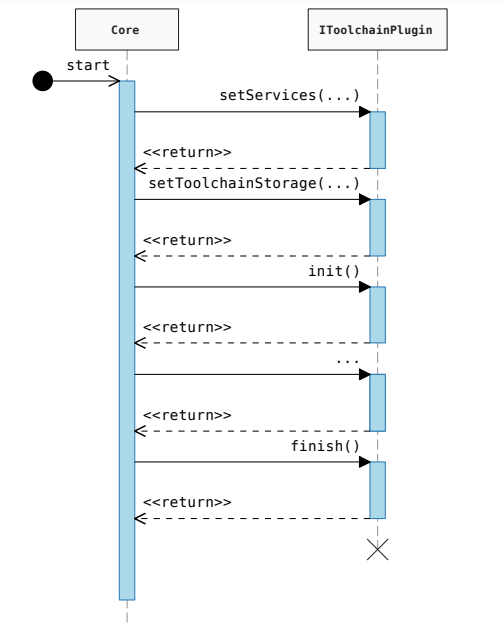
\includegraphics[scale=0.425]{pluginLifecycle.png}
        \caption{The lifecycle of a toolchain plugin as UML sequence chart. All toolchain plugins share this lifecycle, but differ between the calls to \code{init()} and \code{finish()}.
		}
    \end{figure}    
\end{frame}

\begin{frame}{Ultimate's intermediate verification language}
	\begin{itemize}
		\item \ultimate contains its own intermediate verification language, an extension of the Boogie intermediate verification language.
		\item  Boogie is particular suitable to verification tasks because it allows for easy modelling of arbitrary types as well as non-deterministic values and control-flow. 
		\item Most of \ultimates toolchains first encode some verification problem, usually the correctness of an input program, as a Boogie program.
		\item Next, the plugin \code{BoogiePreprocessor} is used to simplify such a Boogie program.
	\end{itemize}
\end{frame}

\begin{frame}{Plugin : BoogiePreprocessor}
	\begin{itemize}
		\item \code{BoogiePreprocessor} first performs type checking on its input. It then replaces many constructs by simpler ones.
		\item For example, it flattens structs to normal variables, inlines constants and functions, and unstructures the controlflow. Unstructuring the control-flow means transforming the AST such that \code{while}, \code{if}, and \code{break} statements are replaced with blocks containing one label statement at the beginning, some sequence of \code{assert}, \code{assume}, assignment, \code{havoc}, or \code{call} statements in between and ending with either a single \code{goto} or a single \code{return} statement.
	\end{itemize}
\end{frame}

\begin{frame}{Plugin : RCFGBuilder}
	\begin{itemize}
		\item Next, the plugin \code{RCFGBuilder} uses the preprocessed Boogie program to create an interprocedural or \textbf{recursive control flow graph}.
		\item A recursive control flow graph (RCFG) is a tuple $R = (Loc, Loc_{init}, Loc_{error}, E, st)$ where
		\begin{itemize}
			\item $Loc$ is a set of program locations,
			\item $Loc_{init} \subseteq Loc$ is a set of initial program locations,
			\item $Loc_{error} \subseteq Loc$ is a set of program locations that violate a specification,
			\item $E \subseteq \mathnormal{P}(Loc) \times Loc$ is a transition relation and
			\item $st : E \to Stmt$  is a labeling function that labels each transition with a statement $s$, where $s$ is either an assignment, an assume, a havoc, a call, or a return.
		\end{itemize}
		\item An element $e$ of $E$ is an ordered pair $(S, t)$, where $S$ is the non-empty set of source locations of $e$ and $t$ is the target location. The size of $S$ is restricted to two locations, i.e., $|S| \leq 2$.
	\end{itemize}
\end{frame}

\begin{frame}{Plugin : RCFGBuilder (cont'd)}
	\begin{itemize}
		\item For each procedure $p$, an RCFG contains the control flow graph of $p$, which has one entry location $l^{entry}_{p}$ and one exit location $l^{exit}_{p}$.
		\item A transition $e_{p} = (\{l\}, l')$ between locations $l$ and $l'$ of $p$ is labeled with either assume, assignment, or havoc statements.
	\end{itemize}
\end{frame}

\begin{frame}{Plugin : RCFGBuilder (cont'd)}
	\begin{itemize}
		\item Calls and returns between two procedures $p$ and $q$ are encoded as follows.
		\begin{itemize}
			\item A call from $p$ to $q$ is a transition $e_{call} = (\{l_{p}\}, l^{entry}_{q})$ from a location $l_{p}$ in $p$ to the entry location $l^{entry}_{q}$ in $q$. $e_{call}$ is labeled with a call statement.
			\item A return from $q$ to $p$ has to correspond to some former call of $q$ from $p$. Hence, a return from $q$ to $p$ is a transition $e_{return} = (\{l^{exit}_{q}, l_{p}\}, l'_{p})$ from the exit location of $q$ and the corresponding call location $l_{p}$ in $p$ to the call successor location $l'_{p}$ in $p$. $e_{return}$ is labeled with a return statement.
		\end{itemize}
		\item For simplicity, we also say that $(l, stmt, l′)$ is an edge of an RCFG $R$ if there
		exists an edge $e = (S, t)$ in $E$ with $st(e) = stmt$, $l \in S$, and $t = l'$.
	\end{itemize}
\end{frame}

\begin{frame}{Plugin (Controller)}
	\begin{itemize}
		\item \ultimate currently provides five different controller plugins.
		\begin{itemize}
			\item \code{UltimateCLI} is a command-line interface (CLI) for users and runs a single toolchain according to the provided parameters. All of \ultimates releases use this controller.
			\item \code{UltimateGUI} and \code{UltimateTest} are used exclusively by Ultimate developers and are normally not deployed.
			\item \code{CDTPlugin} provides an interface for end users that integrates into Eclipse C/C++ development tooling (Eclipse CDT), an IDE for C and C++ development. It lets users verify their C programs directly from their IDE and also displays resulting error paths like a debugger.
			\item \code{WebInterface} provides an API that can be run in an application server and a JavaScript-based website were users can use different Ultimate-tools and explore their capabilities.
		\end{itemize}
	\end{itemize}
\end{frame}

\begin{frame}{Plugin (Source)}
	\begin{itemize}
		\item \code{BoogieParser} create a Boogie AST from a Boogie program.
		\item \code{CDTParser} uses the Eclipse CDT parser together with the \code{ACSLParser} library to create an ANSI-C AST decorated with ACSL specifications. 
		\item Others : \code{PEAtoBoogie}, \code{SpaceExParser}, \code{AutomataScriptParser}, \code{SmtParser}.
	\end{itemize}
\end{frame}

\begin{frame}{Plugin (Source)}
	\begin{itemize}
		\item \code{BoogieParser} create a Boogie AST from a Boogie program.
		\item \code{CDTParser} uses the Eclipse CDT parser together with the \code{ACSLParser} library to create an ANSI-C AST decorated with ACSL specifications. 
		\item Others: \code{PEAtoBoogie}, \code{SpaceExParser}, \code{AutomataScriptParser}, \code{SmtParser}.
	\end{itemize}
\end{frame}

\begin{frame}{Plugin (Analyzer)}
	\begin{itemize}
		\item Many analyzer plugins perform a source-to-source transformation by modifying an existing Boogie AST:
		\begin{itemize}
			\item \code{ProcedureInliner} inlines non-recursive functions and procedures. It decides what to inline when based on black- and whitelists, heuristics like the number of occurrences of a procedure, or the presence of recursions.
			\item \code{BoogiePreprocessor} modifies Boogie ASTs by preprocessing them to produce unstructured Boogie.
		\end{itemize}
		\item Other analyzer plugins performs their analysis on RCFGs or traces: \code{LassoRanker}, \code{AbstractInterpretation}, \code{ReachingDefinitions}, \code{IRSDependencies}.
	\end{itemize}
\end{frame}

\begin{frame}{Plugin (Generators)}
	\begin{itemize}
		\item \code{CACSL2BoogieTranslator} translates a C AST to Boogie.
		\item \code{RCFGBuilder} translates unstructured Boogie into an RCFG.
		\item \code{BlockEncoding} allows to perform different types of block encoding on RCFGs.
		\item \code{LTL2Aut} and \code{BuchiProgramProduct} implement the encoding of Büchi programs, which are needed for LTL software model checking. \code{LTL2Aut} uses an external tool to create a Büchi automaton from an LTL specification, and \code{BuchiProgramProduct} combines this Büchi automaton with the RCFG of a program.
		\item Another class of generators are actually implementations of various model checking algorithms, which all generate additional models for debugging purposes. \code{TraceAbstraction} implements trace abstraction, an automata-based approach to software model checking used in \ultimate \automizer.
	\end{itemize}
\end{frame}

\begin{frame}{Plugin (Output)}
	\begin{itemize}
		\item \ultimates four output plugins are mostly used for debugging purposes.
		\item \code{BoogiePrinter} prints the last Boogie AST model to a file or to a logger.
		\item \code{CfgPrinter} prints a graph-based model in the DOT language, so that the model can be visualized by various third-party tools.
		\item \code{JungVisualization} works only together with GUI controller plugins and provides a new Eclipse RCP view in which models can be visualized as interactive graph. 
		\item \code{WitnessPrinter} uses \ultimates result and backtranslation services to print violation and correctness witnesses to a file or to a logger.
	\end{itemize}
\end{frame}

\begin{frame}{Plugin (Internal Libraries)}
	\begin{itemize}
		\item \code{GuiLoggingWindow} and \code{GuiGeneratedPreferencePages} are plugins used in the \code{UltimateGUI} controller.
		\item \code{ACSLParser} contains the parser for ACSL that is by the source plugin \code{CDTParser}.
		\item \code{LibModelCheckerUtils} contains various utilities that simplify working with formulas.
		\item \code{LibUltimateUtil} similarly contains utilities for working with \ultimates data structures like graphs and result objects. It also contains different data structures like, e.g., hash relations, union-find maps, differently sized tuples, etc.
		\item \code{LibAutomata} is an automata library that offers data structures and operations to represent and work with different types of automata.
	\end{itemize}
\end{frame}

% ===================== Chapter 8 begin ==================== 

\begin{frame}{B\"uchi Program and B\"uchi Program Product}
  	\begin{itemize}
		\item B\"uchi program is a program which is extended by a fairness constraint.
		\item We show that the problem whether a program satisfies an LTL property can be reduced to the problem whether a B\"uchi program has a fair program execution.
		\item Definition (B\"uchi program)
		\begin{itemize}
			\item A B\"uchi program $B$ = ($Stmt$, $Loc$, $\delta$, $l_{0}$, $Loc_{fair}$) is a program P = ($Loc$, $\delta$, $l_{0}$) whose set of statements is $Stmt$, with a distinguished subset of locations $Loc_{fair}$ $\subseteq$ $Loc$.
			\item We call the locations $Loc_{fair}$ the fair locations of $B$.
		\end{itemize}
  	\end{itemize}
\end{frame}

\captionsetup[figure]{font=scriptsize ,labelfont=scriptsize}
\begin{frame}{B\"uchi Program and B\"uchi Program Product}
    \begin{figure}
        \centering
        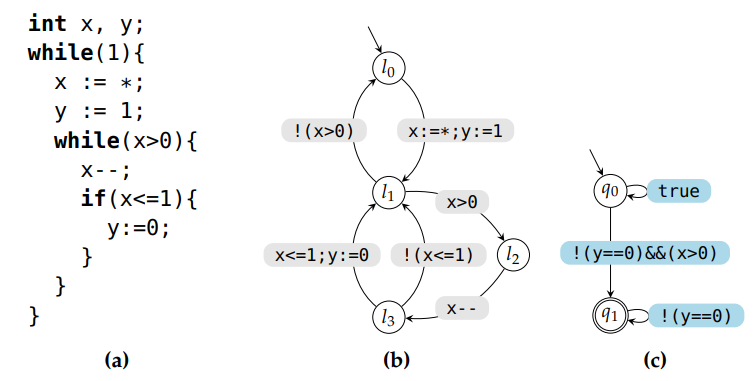
\includegraphics[scale=0.35]{program_and_spec.png}
        \caption{Program P is shown in (a) as Boogie code and in (b) as control flow graph. The B\"uchi automaton $A_{\neg\varphi}$ that represents the negation of the LTL property $\varphi$ = (x > 0 $\rightarrow$ $\Diamond$(y = 0)) is shown in (c).}
    \end{figure}    
\end{frame}

\captionsetup[figure]{font=scriptsize ,labelfont=scriptsize}
\begin{frame}{B\"uchi Program and B\"uchi Program Product}
    \begin{figure}
        \centering
        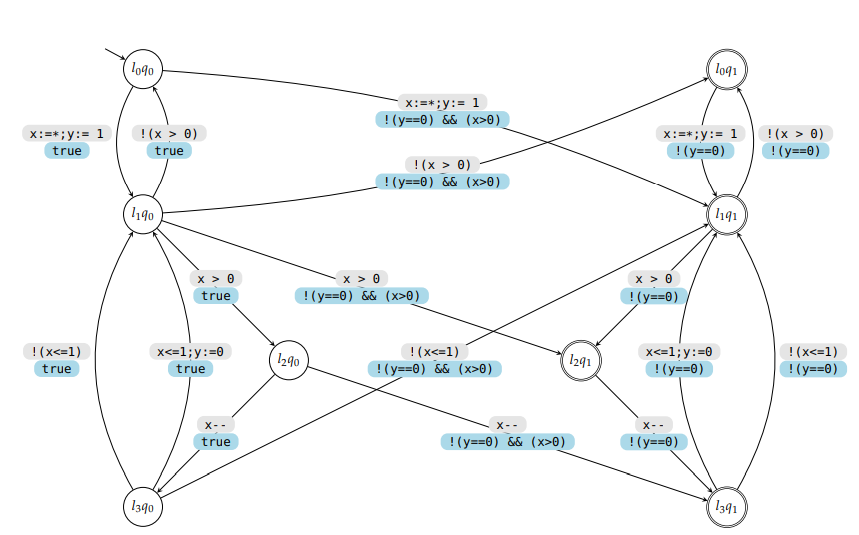
\includegraphics[scale=0.35]{Buchiprogram.png}
        \caption{The B\"uchi program B constructed from the program $P$ and the B\"uchi automaton representing $\neg\varphi$. Each edge is labeled with the statements $s_{1}$ $s_{2}$, where $s_{1}$ comes from $P$ and $s_{2}$ comes from $\neg\varphi$. The fair locations are $l_{0}q_{1}$, $l_{1}q_{1}$, $l_{2}q_{1}$ and $l_{3}q_{1}$, i.e., all locations that contain the B\"uchi automaton’s accepting state $q_{1}$.}
    \end{figure}    
\end{frame}


\begin{frame}{B\"uchi Program and B\"uchi Program Product}
  	\begin{itemize}
		\item Definition (Fair trace)
		\begin{itemize}
			\item A trace $s_{0}s_{1}s_{2}\cdots$ of a B\"uchi program $B$ is a fair trace if
			\begin{itemize}
				\item there exists a sequence of locations $l_{0}l_{1}\cdots$ such that $l_{0} \xrightarrow{s_{0}} l_{1} \xrightarrow{s_{1}} l_{2} \xrightarrow{s_{2}} \cdots$ is a path in $B$, i.e., ($l_{i},s_{i}, l_{i+1}) \in \delta$ for i = 0, 1, $\cdots$, and
				\item the sequence $l_{0}l_{1}\cdots$ contains infinitely many fair locations.
			\end{itemize}
		\end{itemize}
		\item We use $T_{fair}(B)$ to denote the set of fair traces of $B$.
  	\end{itemize}
\end{frame}

\begin{frame}{B\"uchi Program and B\"uchi Program Product}
  	\begin{itemize}
		\item If we consider the B\"uchi program $B$ = ($Stmt$, $Loc$, $\delta$, $l_{0}$, $Loc_{fair}$) as a B\"uchi automaton where
		\begin{itemize}
			\item the alphabet is the set of program statements $Stmt$
			\item the set of states is the set of program locations $Loc$
			\item the transition relation is the labeled edge relation $\delta$ 
			\item the initial state is the initial location $l_{0}$
			\item the set of accepting states is the set of fair locations $Loc_{fair}$
		\end{itemize}
		\item The language of this B\"uchi automaton is exactly the set of fair traces of the B\"uchi program.	
  	\end{itemize}
\end{frame}

\begin{frame}{B\"uchi Program and B\"uchi Program Product}
  	\begin{itemize}
		\item Definition (Fair program execution)
		\begin{itemize}
			\item A program execution $\pi$ of a B\"uchi program $B$ is a fair program execution of $B$ if $\pi$ is the program execution of some fair trace of $B$. 
			\item We use $\prod_{fair}(B)$ to denote the set of all fair program execution of $B$.
		\end{itemize}
		\item We note that traces that are fair and feasible have at least one fair program execution.
		\item For a letter a $\in$ 2 AP, we will use \textbf{assume a} to denote the assume statement whose expression evaluates to true for each state $\sigma$ that satisfies a. 
		\item Hence \textbf{assume a} has the following successor relation:\\ \{($\sigma$, $\sigma$\textquotesingle) $\mid$ $\sigma$ $\models$ p for each p $\in$ a\}
  	\end{itemize}
\end{frame}

\begin{frame}{B\"uchi Program and B\"uchi Program Product}
  	\begin{itemize}
		\item Definition (B\"uchi program product)
		\begin{itemize}
			\item Let $P$ = ($Loc$, $l_{0}$, $\delta_{P}$) be a program over the set of statements $Stmt$
			\item AP is a set of atomic propositions over the program’s variables $Var$.
			\item Let A = ($\Sigma$, $Q$, $q_{0}$, $\rightarrow$, $F$) be a B\"uchi automaton whose alphabet is $\Sigma$ = $2^{AP}$.
			\item The B\"uchi program product P $\otimes$ A is a B\"uchi program $B$ = ($Stmt_{B}$, $Loc_{B}$, $l_{{0}_{B}}$, $\delta_{B}$, $Loc_{{F}_{B}}$) such that the set of statements consists of all sequential compositions of two statements where the first element is a statement of $P$ and the second element is a statement that assumes that a subset of atomic propositions is satisfied, i.e.,\\
			$Stmt_{B}$ = \{s; \textbf{assume a} $\mid$ s $\in$ $Stmt$, a $\in$ $2^{AP}$\}

		\end{itemize}
  	\end{itemize}
\end{frame}

\begin{frame}{B\"uchi Program and B\"uchi Program Product}
  	\begin{itemize}
		\item Definition (B\"uchi program product)
		\begin{itemize}
			\item the set of locations is the Cartesian product of program locations and B\"uchi automaton states, i.e.,\\
			$Loc_{B}$ = \{($l$, $q$) $\mid$ $l$ $\in$ $Loc$ and $q$ $\in$ Q\}
			\item the initial location is the pair consisting of the program’s initial location and the B\"uchi automaton’s initial state, i.e.,\\
			$l_{{0}_{B}}$ = ($l_{0}$, $q_{0}$)
			\item the labeled edge relation is a product of the program’s edge relation and the transition relation of the B\"uchi automaton such that an edge is labeled by the statement that is a sequential composition of the program’s edge label and an assume statement obtained from the transition’s letter, formally defined as follows:\\
			 $\delta_{B}$ = \{(($l$, $q$),s; \textbf{assume a},($l$′, $q$′)) $\mid$ ($l$,s, $l$′) $\in$ $\delta_{P}$ and ($q$, a, $q$′) $\in$ $\rightarrow$\}
		\end{itemize}
  	\end{itemize}
\end{frame}

\begin{frame}{B\"uchi Program and B\"uchi Program Product}
  	\begin{itemize}
		\item Definition (B\"uchi program product)
		\begin{itemize}
			\item the set of fair locations contains all pairs where the second component is an accepting state of the B\"uchi automaton, i.e., \\ $Loc_{{F}_{B}}$ = {($l$, $q$) $\mid$ $l$ $\in$ $Loc$ and $q$ $\in$ $F$}.
		\end{itemize}
		\item The following theorem shows how we can use the B\"uchi program product to check if a program satisfies an LTL property.
		\begin{theorem}
			The program $P$ satisfies the LTL property $\varphi$ if and only if the Büchi program product $B$ = $P$ $\otimes$ A$\neg\varphi$  does not have a trace that is fair and feasible, i.e.,\\
			$P$ $\models$ $\varphi$ iff $T_{fair}$(B) $\cap$ $T_{feas}(B)$ = $\emptyset$
		\end{theorem}
		\item We conclude that the intersection $T_{fair}$(B) $\cap$ $T_{feas}(B)$ is empty if and only if each program execution of $P$ satisfies the LTL property $\varphi$.
  	\end{itemize}
\end{frame}


% ===================== Chapter 8 end ====================

\begin{frame}{Reference}
	\begin{itemize}
		\item Ultimate website\\
		\ultimateURL
		\item Daniel Dietsch : Automated verification of system requirements and software specifications. 2016.\\
		\url{https://freidok.uni-freiburg.de/data/11159}
	\end{itemize}
\end{frame}



\end{document}